\section{Comportamiento}
\label{seccion-comportamiento-apis}
A continuación se describe el comportamiento de las acciones disponibles en las APIs de alto nivel, utilizando diagramas de actividades. Se agruparon estas acciones según su nivel de interacción con las diferentes capas de abstracción de la solución. Las capas de abstracción corresponden: a la API de alto nivel, el Servidor WebSocket, las instancias de la clase OpenGloveDevice en el servidor, la instancia de LegacyOpenGlove (API C\# de bajo nivel) y el software de control Arduino. 

\subsection{Acciones sobre APIs de alto nivel} 
\begin{figure}[H]
  \begin{center} 
   	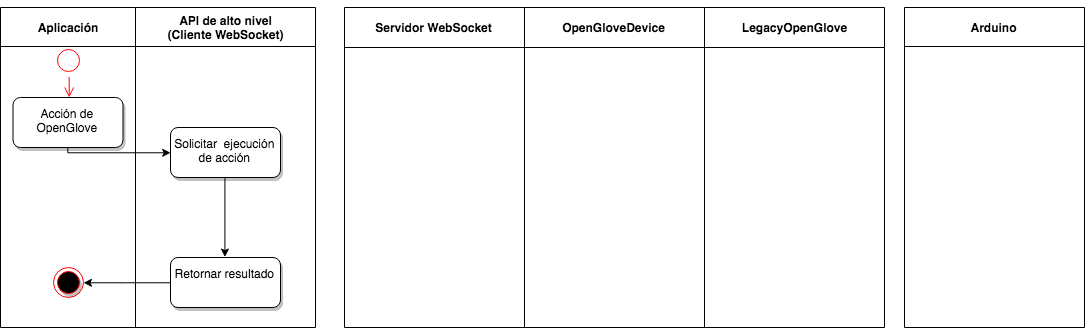
\includegraphics[width=1.0\textwidth]{images/chapter04/ActivityDiagrams-OpenGloveActions-0.png} 
   	\captionsetup{justification=centering}
    \caption[Diagrama de actividades de las acciones OpenGlove sobre APIs de alto nivel]{Diagrama de actividades de las acciones OpenGlove sobre APIs de alto nivel \\Fuente: Elaboración propia (2018)}
    \label{fig:activity-diagrams-0-api-hl}
  \end{center}
\end{figure}


\subsection{Acciones sobre servidor WebSocket}
\begin{figure}[H]
  \begin{center} 
   	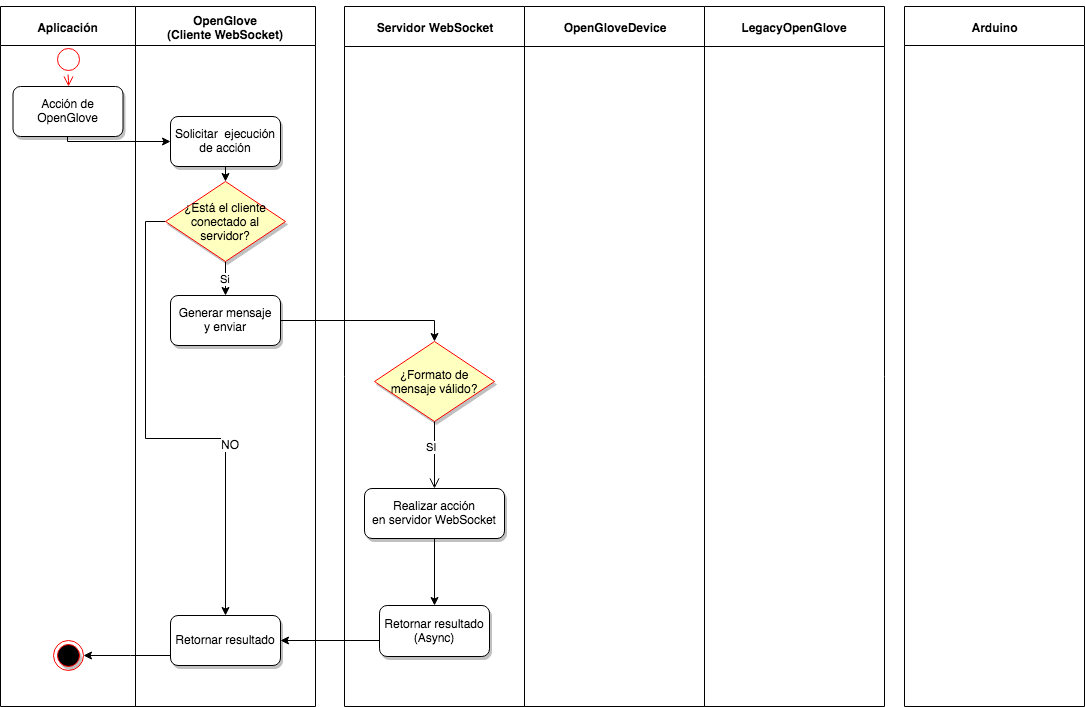
\includegraphics[width=1.0\textwidth]{images/chapter04/ActivityDiagrams-OpenGloveActions-1.png} 
   	\captionsetup{justification=centering}
    \caption[Diagrama de actividades de las acciones OpenGlove sobre servidor WebSocket]{Diagrama de actividades de acciones OpenGlove sobre servidor WebSocket\\Fuente: Elaboración propia (2018)}
    \label{fig:activity-diagrams-1-websocket-server}
  \end{center}
\end{figure}


\subsection{Acciones sobre instancias de OpenGloveDevice}
\begin{figure}[H]
  \begin{center} 
   	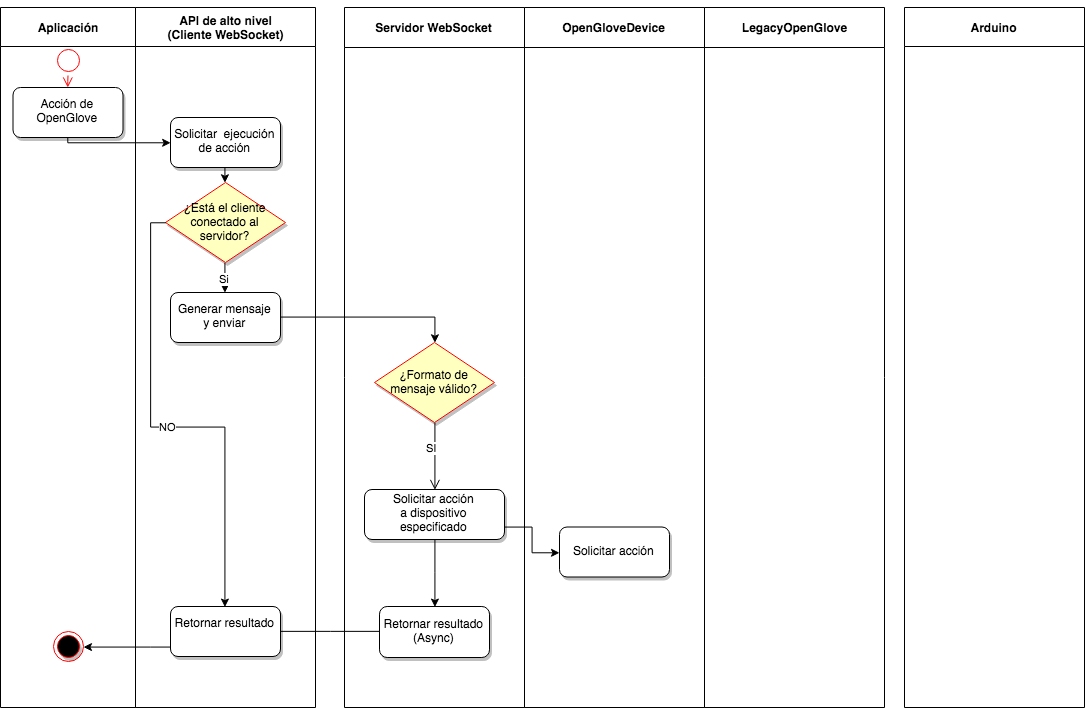
\includegraphics[width=1.0\textwidth]{images/chapter04/ActivityDiagrams-OpenGloveActions-2.png} 
   	\captionsetup{justification=centering}
    \caption[Diagrama de actividades de las acciones OpenGlove sobre instancias de OpenGloveDevice en servidor]{Diagrama de actividades de las acciones OpenGlove sobre instancias de OpenGloveDevice en servidor\\Fuente: Elaboración propia (2018)}
    \label{fig:activity-diagrams-2-openglovedevice}
  \end{center}
\end{figure}



\subsection{Acciones sobre software de control Arduino}
\begin{figure}[H]
  \begin{center} 
   	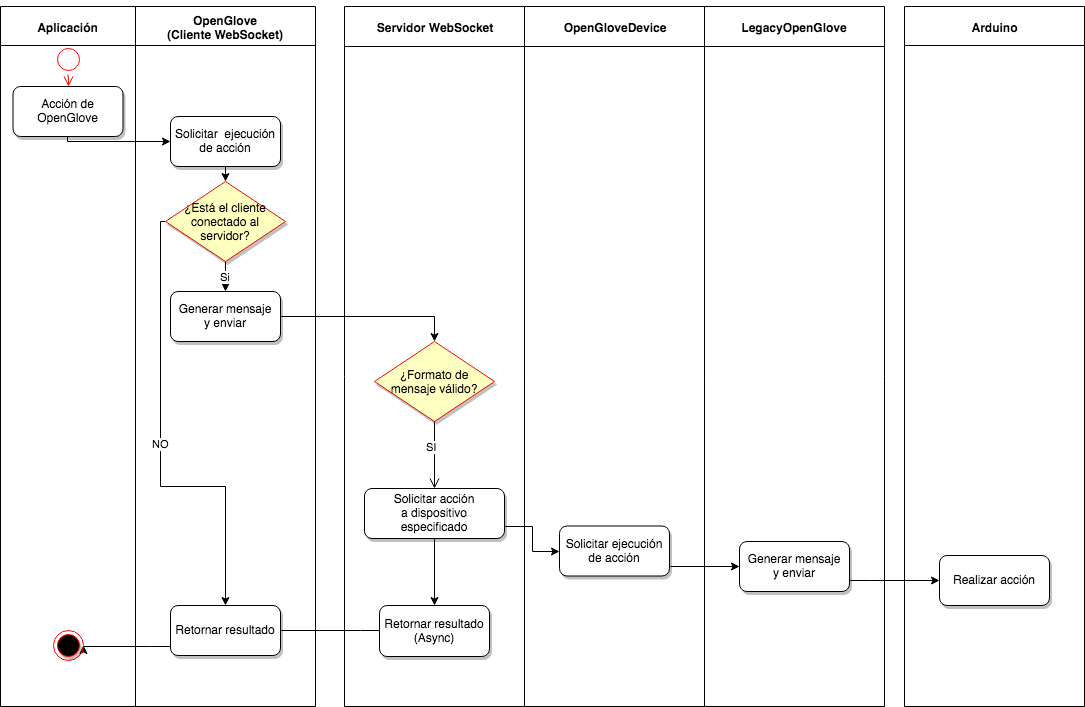
\includegraphics[width=1.0\textwidth]{images/chapter04/ActivityDiagrams-OpenGloveActions-3.png} 
   \captionsetup{justification=centering}
    \caption[Diagrama de actividades de las acciones OpenGlove sobre instancias de OpenGloveDevice en servidor]{Diagrama de actividades de las acciones OpenGlove sobre instancias de OpenGloveDevice en servidor\\Fuente: Elaboración propia (2018)}
    \label{fig:activity-diagrams-3-arduino}
  \end{center}
\end{figure}


\subsection{Lectura de datos provenientes de Arduino}
Este comportamiento ocurre cuando se ha inicializado por lo menos un flexor y/o se ha inicializado la IMU con un valor booleano verdadero (SetIMUStatus). La Figura \ref{fig:activity-diagrams-4-ReadDataFromArduino}

\begin{figure}[H]
  \begin{center} 
   	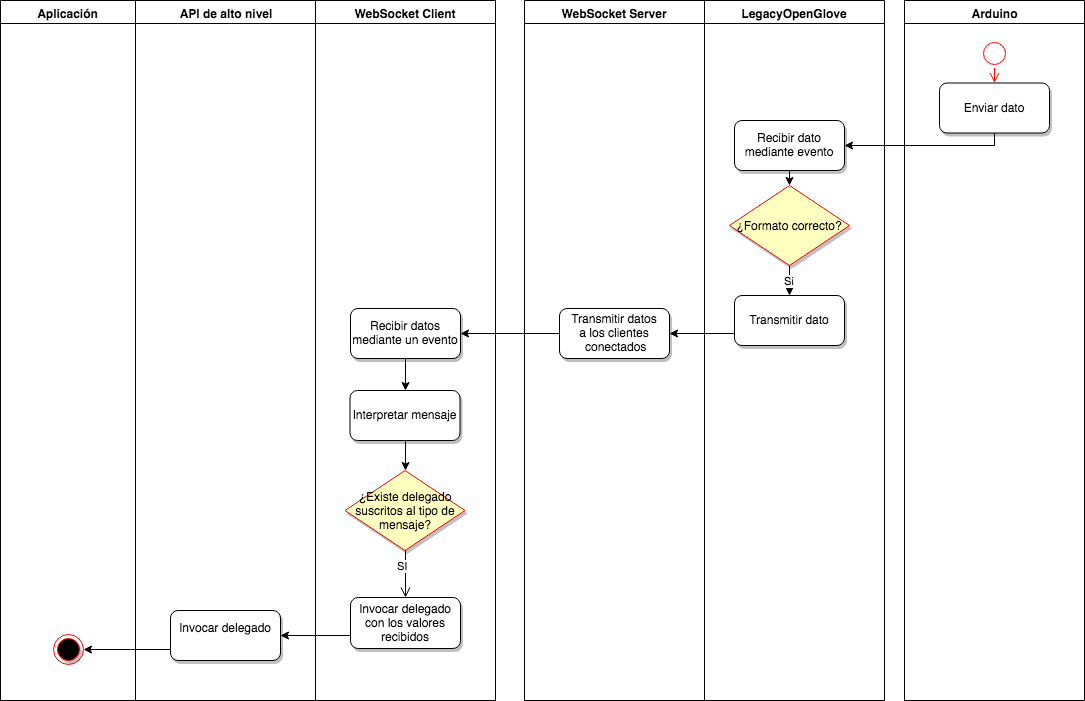
\includegraphics[width=1.0\textwidth]{images/chapter04/ActivityDiagrams-ReadDataFromArduino.png} 
   	\captionsetup{justification=centering}
    \caption[Lectura de datos provenientes de Arduino]{Lectura de datos provenientes de Arduino \\Fuente: Elaboración propia (2018)}
    \label{fig:activity-diagrams-4-ReadDataFromArduino}
  \end{center}
\end{figure}